\section{Integration of large language models}\label{sec:implementation_tools}
Integrating large language models for data clumps refactoring poses the challenge of transmitting source code to the model, and afterwards integrating the changes and  feedback back to the source code. Difficulties arise of how to submit the source code to the \ac{LLM} and  the model should reply so that such integration runs as seamlessly as possible. 

The challenges differ between the concrete uses of the \ac{LLM}. The following applications of models are discussed in this section:
\begin{enumerate}
    \item Detecting data clumps
    \item Choosing the best data clumps
    \item Refactoring data clumps
\end{enumerate}

Each usage can be performed independently from each other, but internally all previous steps must be conducted. For instance, a model instructed to refactor data clumps must find them first, then decide which data clumps are worthy to refactor (these could be all data clumps), and then refactor them. Similarly, a model instructed to filter data clumps must find them first, but does not need to refactor them.

\subsection{Input processing}

\begin{table}[ht!]
    \centering
    \begin{tabular} {m{4cm} | m{4cm} | m{4cm}}
        Detecting & Filtering & Refactoring  \\\hline
         \begin{itemize}
             \item AST
             \item Full source code 
             \item Snippets of methods with at least three parameters, classes with at least three fields
         \end{itemize} & \begin{itemize}
             \item Data Clump Type Context
             \item Full source code
             \item Snippets of source code of the data clumps
         \end{itemize} & \begin{itemize}
             \item Full source code 
             \item Snippets of source code of the data clumps
         \end{itemize}
    \end{tabular}
    \caption{Input categories for different scenarios regarding using \ac{LLM} in data clump refactoring}
    \label{tab:data_clump_llm_input}
\end{table}

The input provided to a model is strongly dependent on the purpose of the model. Table \ref{tab:data_clump_llm_input} shows possible input types for each \ac{LLM} usage. Each input type is discussed below:

\subsubsection{AST}

The \ac{AST} is an effective method to give the model all relevant information about the source code.  The \ac{AST} only contains a reduced structure of the source code and will therefore help to reduce processing cost. However, the \ac{AST} is usually not directly available but must be produced by other tools or ChatGPT (which means the source code has to be sent to the \ac{LLM} nevertheless). Additionally, there is no fixed format for the \ac{AST} which might complicate parsing and processing the \ac{AST} or the results by ChatGPT.

If ChatGPT is also tasked with refactoring, using \ac{AST} may not be as beneficial. Refactoring often involves updating method calls or variable usages, which may not be fully represented in the \ac{AST}. One could hypothetically submit both the \ac{AST} and the source code, enabling ChatGPT to use the \ac{AST} for detection and the source code for refactoring. However, this approach increases costs and it is unclear whether it could degrade the quality since ChatGPT would need to process more data and establish a correlation between the source code and the \ac{AST}.

\subsubsection{Full source code}

An expensive method that works with all three application of \acp{LLM} is providing the full source code. This means that the source code is transmitted to the model without any modification. While the overhead is large, this method gives the model the largest amount of information so that it might execute the detection, filtering, or refactoring step more reasonably. However, due to context size limitation and resource allocation, providing large files can have a detrimental  effect on the quality. 

\subsubsection{Code snippets}


Another possible approach is to only provides those lines of code that relate to data clumps. As a result, only parts of the source code are transmitted which can save many tokens and helps the model to focus on the relevant parts. These lines might be called \textbf{relevant locations}



The major issue with this strategy is to choose which lines of code to transmit. Only if the data clumps are already known, all relevant location can be found and transmitted to the model. This does not work if it is the purpose of the model to also to detect data clumps. In this case, one strategy could be to define the locations of interest as lines where either a method with at least three parameters is declared, or a field in a class with at least three fields is declared. This ensures that only potentially relevant lines are considered.

Artificially enlarging the number of locations of interest is also a method worth discussing. Instead of transmitting only the line of the data clump items,  a small neighborhood or margin around these lines is transmitted, too. This helps the model to gain a better overview about the source code. For instance, these additional lines could include documentation or the usage of variables, thereby helping the \ac{LLM} in its task.

\begin{figure}
    \centering
    \includesvg[width=0.4\columnwidth]{figures/chapter4/margin_effect.drawio.svg}
    \caption{The effect of varying the margin on the available information}
    \label{fig:margin_effect}
\end{figure}

Figure \ref{fig:margin_effect} illustrates the advantage of a larger margin size. The source code shows counters used for testing purposes and a possible way to reset them \footnote{This example is somewhat inspired by a JUnit5 data clump that was refactored as part of the evaluation in section \ref{sec:pull_request_eval}}. The first four fields are part of a data clump (the second class is not shown for brevity). Consider only the data clump item \enquote{afterAll}. If the margin is zero, only line 4 would be transmitted to the model (black rectangle). This means that the \ac{LLM} has only a scarce overview over the purpose of the variable.
The green rectangle covers the area if a margin of one is used. Now, line 3 and 5 are also included. Since line 5 mentions something about tests, the model can infer where the data clump items are used and might improve its refactoring. The red rectangle represents a margin size of three. In this case, the full code block is transmitted, and the model can observe that it might be useful to include a reset method in the extracted class. 

However, not only data clumps items could be used as the starting point of the additional lines. Many source code files contains a header and import statements in the beginning. These information can be beneficial especially in case of refactoring as the model can better understand the types of the variables or the context of the source code.

In this master thesis mainly a constant margin is considered. However, variable margins that depends on the programming language or statistics of the source code (average length of a method or documentation) could be considered too.







\subsection{Output processing}\label{sec:output_processing}
An \ac{LLM} on its own cannot change code or controls a system since, for the purpose of this master thesis, it  can only output textual information. Therefore, each output from the model must be received and interpreted  in order to serialize them permanently. Two approaches are discussed. 

\subsubsection{By human in the loop}
Commonly, the refactoring is done by human beings who review the output, interpret it and use the gained knowledge to simplify the workflow. In the case of refactoring, the model can propose changes to the source code, but cannot change the source code directly. Instead, a human in the loop has to read the refactoring suggestion, determine whether they are reasonable, and perform the suggested refactoring. In the last step, this involves also finding the affected files, change them, and test the changes. Hence, while an \ac{LLM} can help to make decisions, manual work must still be performed. 

One approach to facilitate these suggestions is to create a mirror file. This means that the original file is untouched but the changes are written to a similar named but new file. A human in the loop must then manually apply the refactoring suggested in the mirror file to the original file. While this is a more time-consuming task, it allows for more control by the developer. Additionally, \acs{LLM} tend to omit unchanged code. Directly overwriting files will therefore result in much smaller files that have lost much of their contents. Moreover, creating multiple mirror file would be possible allowing to the developer to have multiple refactoring option suggested by one or multiple models with various parameters so that there is more flexibility. 
Markdown is one common way to integrate code and text description to explain the human in the loop to decide what steps to perform in order to successfully refactor the data clump.  

\subsubsection{Automatically processing}

Automatically processing and applying such refactoring proposals can be more difficult.
First of all they must be parsed in order to be applied. The markdown format can be analyzed automatically by clearly splitting code and text sections, however it is difficult to apply the code section to the correct location. 

As an alternative, the \ac{JSON} format allows for easier automatic processing of the response as \ac{JSON} data can be parsed without major obstacles and can contain all relevant information. For instance, \ac{JSON} data that contains the path to a file as the key, and the file content as its value can be parsed and the file content can be written to the given location. Some \acs{LLM} also allow to force the \ac{JSON} format so that the response is always valid \ac{JSON}, although it might not be in the requested format. 

The disadvantage of \ac{JSON} is that it is harder to read by the human in the loop. Because JSON strings do not support new lines and code files contain many new lines, they are hard to read and understand.
One challenging aspect of this method is that the \ac{LLM} will likely make errors. For instance, the modified files are not compilable as the file might not be complete or the  overwritten files contain explanatory text. A human in the loop must then apply the necessary corrections on the overwritten file.



Therefore, the \ac{JSON} approach should be modified so that not full file contents are returned but replacement instructions. These are instruction given by the model to replace specific lines by a given text, so that only specific lines of a file are modified.  As a result, code lines not related to data clumps can be left untouched minimizing the risk for mistakes. 


Figure \ref{fig:json_based_changes} illustrates how the diff-based approach works on a small example. The original source code on the top-left is changed by applying the \ac{JSON} in the bottom-center. The modified file is shown in the top-right of the figure. The red color indicates removed lines. The concrete changes are as follows:
\begin{figure}
    \centering
    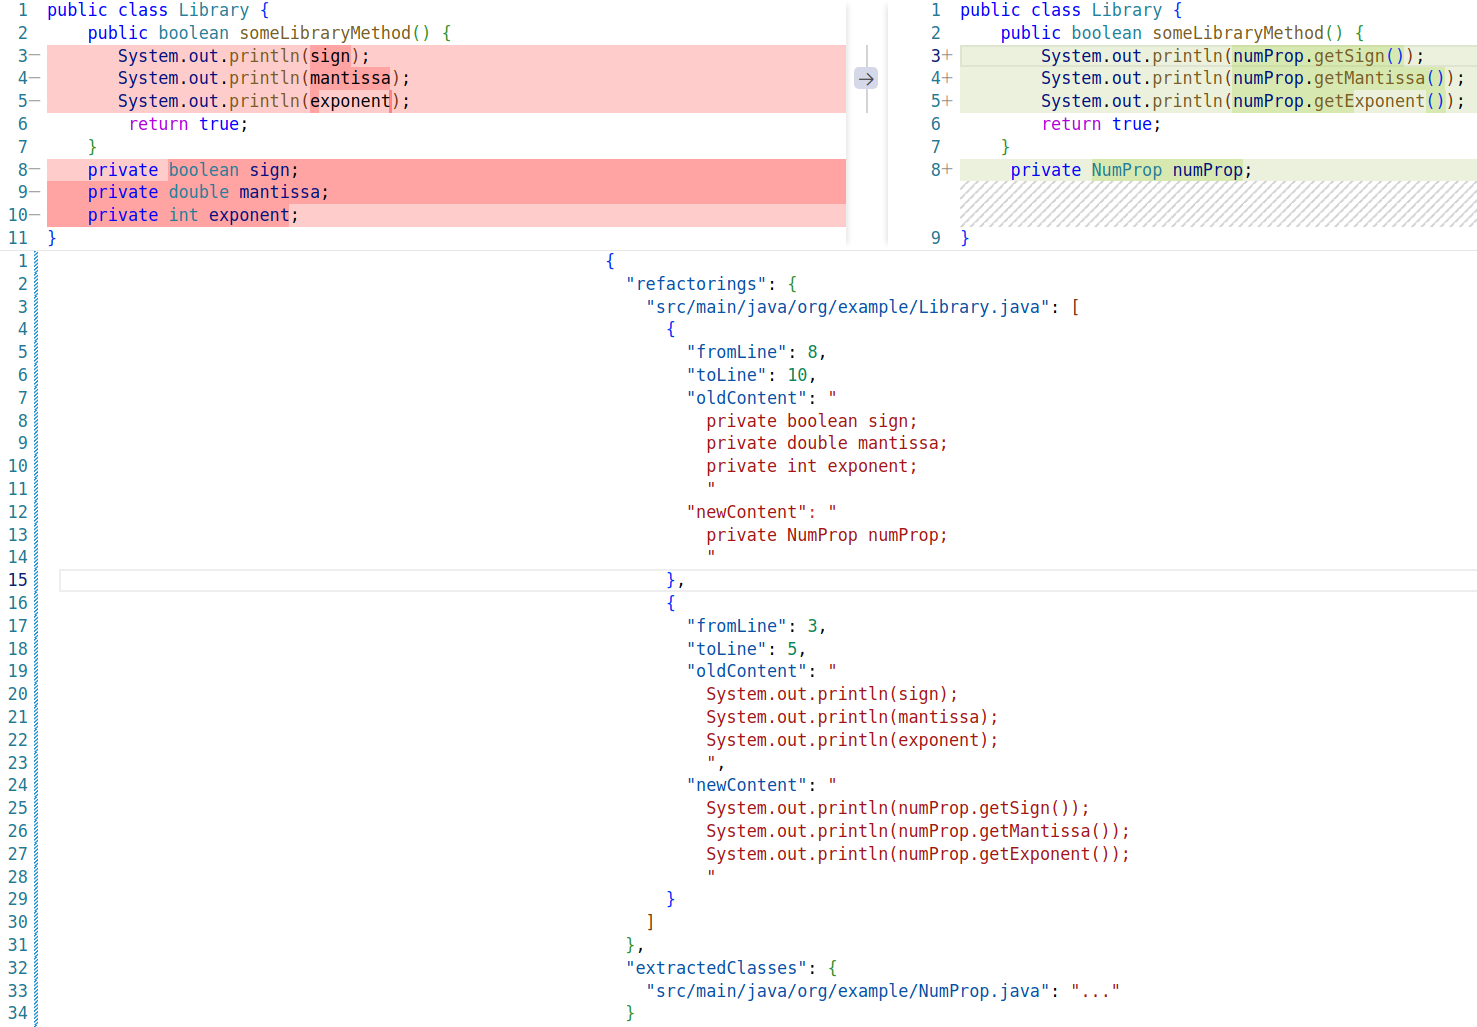
\includegraphics[width=\columnwidth]{figures/chapter4/diff_original_changed_vscode_cmp.png}
    \caption{Diff-based approach applied on a small example}
    \label{fig:json_based_changes}
\end{figure}


\begin{itemize}
    \item In file \enquote{Library.java}
    \begin{itemize}
        \item replace the \textit{oldContent} in line 8-10 of the original file with \textit{newContent}.
        \item => This removes the data clump items
       \item replace the \textit{oldContent} in line 3-5 of the original file with \textit{newContent}.
        \item => This replaces the usages of the data clump item by an object of the extracted class 
    \end{itemize}
    \item Create a new class at the location \enquote{NumberProperties.java} with the specified content. The content is ommitted for brevity
\end{itemize}



One major issue is how to apply the suggested changes. Two approaches are possible.
In the first approach, the content at lines \enquote{fromLine} to \textit{toLine} is replaced by \enquote{newContent}. This can be challenging if \enquote{newContent} has more lines than \enquote{oldContent}. Additionally, even if these  changes are correctly applied, later changes in the same file can become more problematic as the line number information might be outdated. 

Alternatively, a replace method can be used. This means that the string \enquote{oldContent} is replaced by \enquote{newContent} without considering the line number information. This method prevents the issues of the first approach. Additionally, it might refactor more lines that the \ac{LLM} did not refactor for some reasons. If two code lines are equal and one code line needs to be refactored, there is a high probability that the other string should be changed in the same manner. However, this does not work if \enquote{oldContent} for some reason does not exists in the file. For instance, the model might have added extra whitespaces to the old content so that a simple search-and-replace-strategy does not work. Furthermore, if oldContent is an empty string, replacing can lead to file corruption as the replacement operations are not developed for such an scenario. 

In this master thesis both approaches are employed. The second approach is always tested first. If this approach does not work (e.~g. \enquote{oldContent} does not exists in the file, the line-by-line replacement method is used.  

\subsubsection{Handling invalid \ac{JSON} objects}

When using the \ac{JSON} output format, it is essential to deal with edge cases where the ourput is not valid \ac{JSON}. This problem can happen in two scenarios.

Firstly, not all \acp{LLM} support \ac{JSON}-only modes. This means that that the content of the model cannot be forced to contain only \ac{JSON} but might contain additional text that cannot be parsed. While the model used in this thesis supports this ouput mode, it is useful to keep these edge cases in mind. This edge case can be circumvented by finding the first opening curly brace \enquote{\{} in the response and the last closing curly brace \enquote{\}} because the string between is valid \ac{JSON}. As a result, any text before or after the \ac{JSON} is ignored and cut off. 

Secondly, one problem for \acp{LLM} is that they generate token by token and therefore cannot pre-plan their output. Usually, this does not cause problems. 

However, as outlined in section \ref{sec:llm_challenges}, the maximum output size of a model is restricted so that a model cannot generate large output at once. The model can be prompted to continue the output, but this requires additional prompts. Additionally, these interim prompts must be combined into one so that they can parsed.

If the output is \ac{JSON}, this can become problematic as the syntax of \ac{JSON} is intolerant to sudden stops. For instance, if closing curly braces  are missing, usual \ac{JSON} parsers are unable to deal with. 

The easiest solution to this problem is to simple ignore the output as the response was invalid. Such a large output is correlated with a large input so it might be useful to reduce the set of transmitted files. 

However,  one can still try to parse the output as the incomplete \ac{JSON} might still contain relevant data (e.~g. refactoring instructions). While the refactoring is probably incomplete, it might be a good start and possible errors can be fixed in the validation step.

Parsing such incomplete \ac{JSON} is however not trivial. One approach is to to incrementally remove the last character of the string, and then to try appending closing brackets to the string until the result is a valid \ac{JSON}. This is resource extensive as the validity of the \ac{JSON} must be checked repeatedly. Alternatively, a tolerant \ac{JSON} parser could be used, but these are more appropriate for \acp{JSON} with comments or new lines inside strings. 



\subsection{Proposal handling}

One issue that might occur while working with \ac{LLM} is that their output quality can vary. The same prompt can generate various outputs of which some might be useful and some are not useful. This however is also an advantage of \acs{LLM}. Refactoring data clumps can be performed in many different ways and therefore, the first output might not be the best output. 

Two approaches should be distinguished:
\subsubsection{Parallel Proposals}
The model generates multiple independent proposals. This means that in each proposal the model has no memory of its previous proposals. At the end, the best proposal is chosen and applied to the source code.

The issue is determine the \enquote{best} proposal. One approach could be to determine the proposal that causes the least compiler errors. While this idea might be helpful to reduce the manual work to correct errors, it also can tend to produce proposals that change as few code as possible. For instance, refactoring nothing can cause no compiler errors.

As an alternative, one could count the number of changed lines in a proposal and rate proposals with more changes higher than those with fewer changes. This idea rewards proposals that refactor all locations of interests more than proposals that only refactor only a small part of the program while the data clump exists in other known parts too. 


If interaction is possible, there could be also an option to let the user decide.
\subsubsection{Sequential proposals}

With sequential proposals, one conversation is hold and the context is kept so that that the \ac{LLM} does not forget its previous output. Using this idea, not the first proposal is chosen but the last one after the \ac{LLM} has been given enough chances to correct errors.

Handling sequential proposal is therefore a combination of refactoring and validation handlers. At first, the usual refactoring process is performed. This could be a manual refactoring (e.~g. PSI) or a refactoring via an \ac{LLM}. Then, the refactored code is build. If there a building issues (e.~g. compiler errors or failing tests), the model is instructed to fix them. From now on, only the \ac{LLM} performs the refactoring even if a manual approach was used. Then, the code is build again, and the process starts again if there are errors. 



It should be noted that at some point a proposal should be finally chosen as the \ac{LLM} might not always find a solution that compiles even if infinitive steps were available. Similar to a an optimization algorithm, it can be struck into a local optimum and cannot suggest reasonable changes so that the program compiles again.  